%!TEX root = thesis.tex

%:-------------------------- Preamble -----------------------

% Three languages are supported, which will be reflected in the logo on the front page. Pass the appropriate language
% specified as a class option to uit-thesis. Passing any other languages supported by babel will result in the default
% language on the frontpage. If no language is passed, the default is selected.
%  - USenglish (default)
%  - norsk
%  - samin
% The frontpage comes in two variants, Master's thesis and PhD. Master is default, use classoption 'phd' for the PhD version.
\documentclass[USenglish]{uit-thesis}

% Lorem ipsum
\usepackage{lipsum}

\makeglossaries

% Add external glossaryentries
\loadglsentries{acronyms}
\newacronym{api}{API}{application programming interface}\glsunset{api}
\newacronym{2api}{2API}{application programming interface}
\newacronym{d3}{D3}{Data-Driven Documents}
\newacronym{EXIF}{EXIF}{Exchangeable Image File Format}
\newacronym{html5}{HTML5}{version 5 of the HyperText Markup Language standard}

\newglossaryentry{thesis}
{
  name=thesis,
  description={is a document submitted in support of candidature for an
    academic degree or professional qualification presenting the author's
    research and findings
    },
}
\newglossaryentry{lage}
{
  name={long ass glossary entry},
  description={is a long ass entry with a lot of text describing the properties of the glossary entry. Hopefully this spans some lines now.
  },
}


\newcommand{\listdefinitionname}{My list of definitions}
\newlistof{definition}{def}{\listdefinitionname}
\newcommand{\definition}[1]{%
  \refstepcounter{definition}%
  \par\noindent\textbf{The Definition~\thedefinition. #1}%
  \addcontentsline{def}{definition}
    {\protect\numberline{\thechapter.\thedefinition}#1}\par%
}

\begin{document}

%:-------------------------- Frontpage ------------------------

\title{From Physical to Virtual Sensors (PVS)}
%\subtitle{Subtitle}			% Optional
\author{Camilla Stormoen}
\thesisfaculty{Faculty of Science and Technology \\ Department of Computer Science}
\thesisprogramme{INF-3983 Capstone Project in Computer Science … December 2017}
%\ThesisFrontpageImage{example_image.jpg}	% Optional

\maketitle

%:-------------------------- Frontmatter -----------------------
\frontmatter

%\begin{dedication}
%To somebody.

%Fuck you very much.
%\end{dedication}

%\begin{epigraph}
%\epigraphitem{Simplicity is prerequisite for reliability.}{Edsger Dijkstra}
%\epigraphitem{Beware of bugs in the above code;\\I have only proved it correct, not tried it.}{Donald Knuth}
%\end{epigraph}

\begin{abstract}
%\lipsum[2-3]
\begin{description}
\item[W3] Whats wrong with the world? / motivation 1-3 setninger
\item[Architecture - 1-3 setninger]
\item [Design- 1-3 setninger]
\item[Implementation - 1-3 setninger]
\item[Experiments - 1-3 setninger]
\item[Results - 1-3 setninger]
\item[Lessons learned/main conclusion - 1-3 setninger]
\item [Kutt heller etterpaa] 
\end{description}

This dissertation present/describe ...
\end{abstract}


%\begin{acknowledgement}
%\lipsum[4-8]
%\end{acknowledgement}

\tableofcontents

%\listofdefinition
\listoffigures
%\printglossary
%\printglossaries

%:-------------------------- Mainmatter -----------------------
\mainmatter

\chapter{Introduction}
The Arctic tundra in the far northern hemisphere is challenged by climate changes in the world today and is one of the ecosystems that are most affected by these changes \cite{coat2016}. The \textit{Climate-ecological Observatory for Arctic Tundra - COAT} is a long-term research project developed by five Fram Center\footnote{\url{http://www.framsenteret.no/english}} institutions. Their goal is to create robust observation systems which enable documentation and understanding of climate change impacts on the Arctic tundra ecosystems. In autumn 2015, COAT was granted substantial funding to establish research infrastructure which allowed them to start up a research infrastructure during 2016-2020 \cite{coat2016}. 

Every year, COAT deploys several camera traps in eastern Finnmark, Norway for roughly one month during the winter. The main purpose of these cameras is to study predator populations, with especially a focus on the redlisted arctic fox which is the most endagered mammal species in Norway  \cite{coatplan2016}. 
The camera traps are set up to take a time-lapsed photo every fifth minute during day and night which adds up to over 300 000 images per year \cite{methodseco}. Collecting this high volume of images gives Big Data challenges in the ecology field. 
%The images are also manually examined and annotated, which is a enormously exhausting approach that requires months of human labor and resources.

\textbf{Hvordan komme inn på virtuelle sensorer? Og til "this project will develop an abstraction" eller noe lignende...}

In this project we will describe a system that simplifies biologists need  to look at images from different locations in the Arctic tundra in one view...

Assume biologists want to search for image of a specific animal from different locations in the Arctic Tundra. A virtual sensor would locate data from the data storage and then return those images that matches to the biologists request...

%This project will develop an abstraction for virtual sensors, and do a prototype of the abstraction on a set of computers with physical sensors. The purpose is to provide for a more powerful and flexible sensor in the COAT monitoring of the arctic tundra. As such, a fox feeding station is the usage domain to be used for the prototype.


\section{Motivation}
%\textbf{Problem definition: This project investigated ... x, with the purpose of y.}

The motivation  behind this project is that no single sensor may cover the sensing needs, and that sensing needs can change rapidly over time. Consequently, there is a need for sensor fusion, and allow for combining sensors at different computers.

This project will develop an abstraction for virtual sensors, and do a prototype of the abstraction on a set of computers with physical sensors. The purpose is to provide for a more powerful and flexible sensor in the COAT monitoring of the arctic tundra. As such, a fox feeding station is the usage domain to be used for the prototype.

\section{Contributions}
%\textbf{What was the contribution? Ta enten her eller i conclusion? Eller begge steder}

The dissertation makes the following contributions:
\begin{itemize}
\item An introduction to virtual sensors.
\item A description of data set preparation from the camera traps in the Arctic tundra.
\item An implementation and description of a system that fuse raw data from different physical sensors into one virtual sensor.
\item An evaluation of the system.
\end{itemize}

%OTTO: Principles, models, artifact and evaluation of it. Lessons learned/insights. Conclusion

\section{Assumptions}
AVGRENSE, VIKTIG!!
Something about motivation and stuff

\section{Limitations}
AVGRENSE, VIKTIG!!

\begin{itemize}
\item Mention focus on camera-sensors/data, and not other sensors?!
\item Hvorfor fokus på bilder - forenkle, begrense, starte et sted
\item Limiting search for animals - "predefined" what user can search
\end{itemize}


%Instead of supporting all possible services, we give a predefined..


%\begin{itemize}
%\item The first item .
%\end{itemize}
%\begin{enumerate}
%\item The first item
%\end{enumerate}
%\begin{description}
%\item[Entry A] with definition A.
%\end{description}
%\newpage


\iffalse
\subsection{A subsection - example}
We can use the \ac{api} to \ac{2api} do stuff, and write about what we did in a \gls{thesis}!

This is some stuff, {\sc smallcaps {\em smallcapsemphasized}} {\em regularemphasized}

\Gls{lage}: a test glossary entry.

If the acronym \ac{uit} is displayed, then loadglsentries works.
Hello.

It is fun to use modern \upsc{OpenMP} technology!\footnote{This is a snarky footnote. Words and etc. Semantic web technologies are technologies that enable semantification of the Web as we know it today. Hopefully this spans some lines now.}

It is fun to use \emph{modern \upsc{OpenMP}} technology! And it is fun to use \ac{d3} and \ac{html5}.

Referencing figure \ref{fig:ex} to test link.\footnote{This is another
footnote.}

\definition{Some other definition}
\fi








\chapter{Related Work}
Sensors are becoming omnipresent in everyday life and is generating data at an remarkable rate and scale \cite{modelling}. Sensors and models play a vital role in harnessing "Big Data" to extract information.
% and to illustrate current developments and identify key research needs using human and environmental health challenges as an example. 
As more data become available from sensors, it will require rethinking of the scales, the processed models and creative thinking about fusing data.


The arrival of new instrumentation and sensors has led to an increasing amount of data which are becoming available for researchers and practitioners. However, accessing and integrating these data into usable environment for analysis and modeling can be highly time-consuming and challenging, particularly in real time \cite{hill}.
%It is a prototype of a virtual sensor system for environmental observation with real-time customization of physical sensor data\cite{hill}.
As a solution to this challenge, they developed a prototype where users can exploit deployed virtual sensor types and interactively create and share new customized virtual sensors at different locations and suitable parameters to the researcher's desire.
The system can provide point-averaged radar-rainfall products at either temporal resolution of the radar or as a temporal average of a fixed time period, which is illustrated in Figure \ref{fig:rainfall_sensor}
In contrast, our virtual sensors system is running on-demand, not in real-time. Our approach has neither the ability to provide users to create and share new customized virtual sensor. 

\begin{figure}
\centering
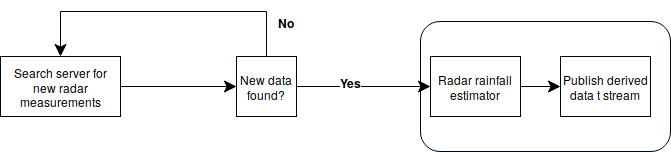
\includegraphics[width=\textwidth]{rainfall_sensor.png}
\caption{Figure illustrating the virtual rainfall sensor.}
\label{fig:rainfall_sensor}
\end{figure}


%\section{Virtual Sensors}
A virtual sensor is a constructed sensor in contrary to a physical sensor \cite{VirtualSensors2006}. They are used in place of the real sensors where they read real physical sensor data and calculate the outputs by using some processing models.

Previous research have focused on simple in-network data aggregation techniques and the sensor networks are often represented as a database. Two examples of such approaches are TinyDB \cite{tinyDB} and Cougar \cite{cougar}, which enable applications to have a central point (base station) and create routing trees  to funnel replies back to this root. The main focus on these approaches are operating intelligent in-network aggregation and routing to reduce  the overall energy cost.
%while still keep the semantic value of data high.
In both examples, the data aggregation is specified using an SQL-like language. However, queries cannot be used to merge different data types, only homogeneous data aggregation is achievable.
Their virtual sensors approach is  offering a simple interface and heterogeneous in-network data aggregation. Our virtual sensors have no SQL-like language or a database to store the aggregated data. Our work also fuses physical sensor data which is already in a data storage, and not consuming directly from the physical sensors.


A virtual node\cite{Ciciriello} is a development of a set of physical sensors that a programmer can interact with as a single sensor. Their virtual nodes are implemented using TinyOS \cite{TinyOS} and is specified using logical neighborhoods \cite{Mottola2006}\cite{Mottola2006_2}. 
%Their physical nodes are abstracted and specified using logical neighborhoods \cite{Mottola2006}\cite{Mottola2006_2}.
The nodes in the logical neighborhood are specified based on their characteristics by the programmer.
Our approach of virtual sensors are not specified by the use of logical neighborhoods. There are no communication between the virtual nodes.




%\subsection{dice - expand!}
Dice?? \cite{dice}
%\textit{"Improve network lifetime -> routing protocol for many-2-many communication". Talking about TinyOS and CTP.
%In this article we present DICE, a system enabling WSN-based distributed monitoring of global invariants. A DICE invariant is expressed by predicates defined over the state of multiple WSN nodes, such as the expected state of actuators based on given sensed environmental conditions.}

\textit{FROM PAPER: We presented DICE (Distributed Invariant CheckEr), a system for WSN-based distributed monitoring of global invariants in physical processes. DICE provides a declarative language to specify invariants and a runtime support enabling efficient monitoring of their violations.}

%\textit{\textbf{SYSTEM ARCHITECTURE}
%We describe the toolchain and runtime architecture of DICE. Our prototype targets TinyOS [Hill et al. 2000]\cite{TinyOS}, and relies on CTP [Gnawali et al. 2009 - Collection tree protocol: two principles of wireless routing protocols] for the tree-based forwarding necessary to the TREE dissemination strategy. Nevertheless, the techniques we describe do not depend on either.
%We use our TinyOS implementation of DICE, described in Section 4, to run both simulation and tested experiments.
%In computer science, an invariant is a condition that can be relied upon to be true during execution of a program, or during some portion of it. It is a logical assertion that is held to always be true during a certain phase of execution.}


%\textit{\textbf{Sensor-Cloud Infrastructure}
%Physical Sensor Management with Virtualized Sensors on Cloud Computing
%http://ieeexplore.ieee.org/document/5635688/\#}




\chapter{The Dataset} \label{chap:data_set}
%\textbf{HVORDAN DE ER SAMLET, HVORDAN DE ER ORGANISERT?}

The dataset is provided by COAT and contains over 1.6 millions of pictures taken from 2011 to 2015 by their camera traps stationed in the Arctic Tundra in Finnmark, Norway. The wildlife camera traps from Reconyx are placed at six different areas in the Arctic Tundra: Nordkynn, Ifjord, Komag, Nyborg, Stjernevann and Gaissene.
The dataset contains pictures during night- and daytime. The cameras have infrared flash so the cameras can take pictures at nighttime. These pictures are without color while the pictures taken at daytime are with color, as shown in Figure \ref{fig:pictures}.

\begin{figure*} %[t!]
    \centering
    \begin{subfigure}[t]{0.45\textwidth}
        %\centering
        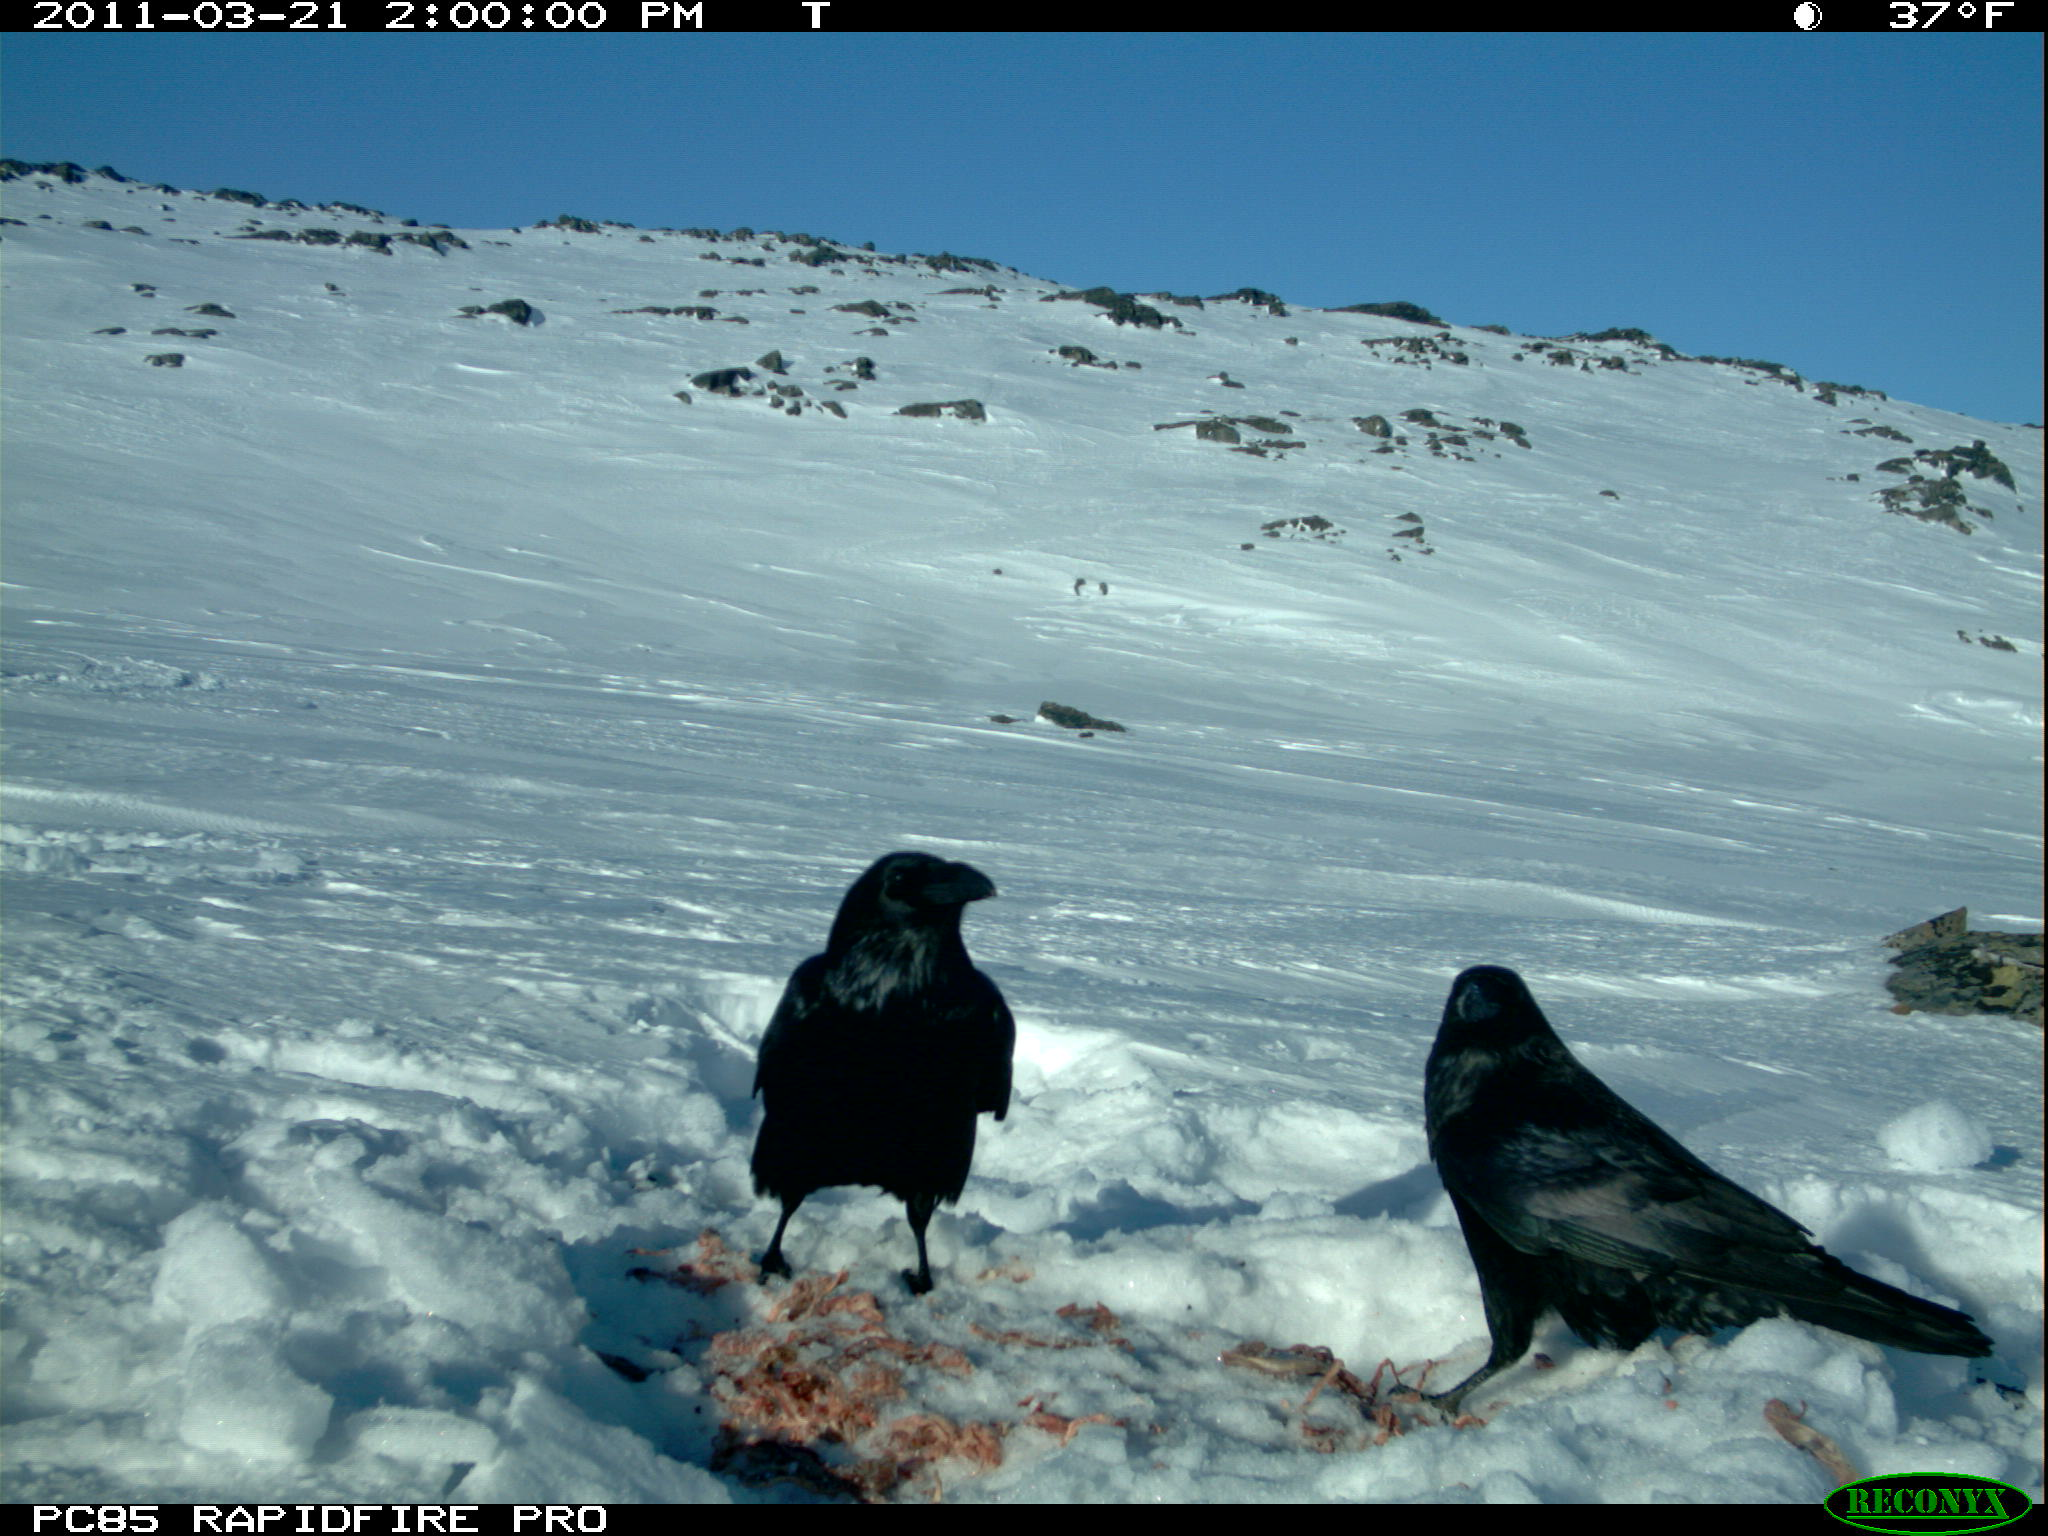
\includegraphics[width=\textwidth]{IMG_0040.JPG}
        \caption{Picture of ravens at daytime.}
    \end{subfigure}%
    ~ 
    \begin{subfigure}[t]{0.45\textwidth}
        %\centering
        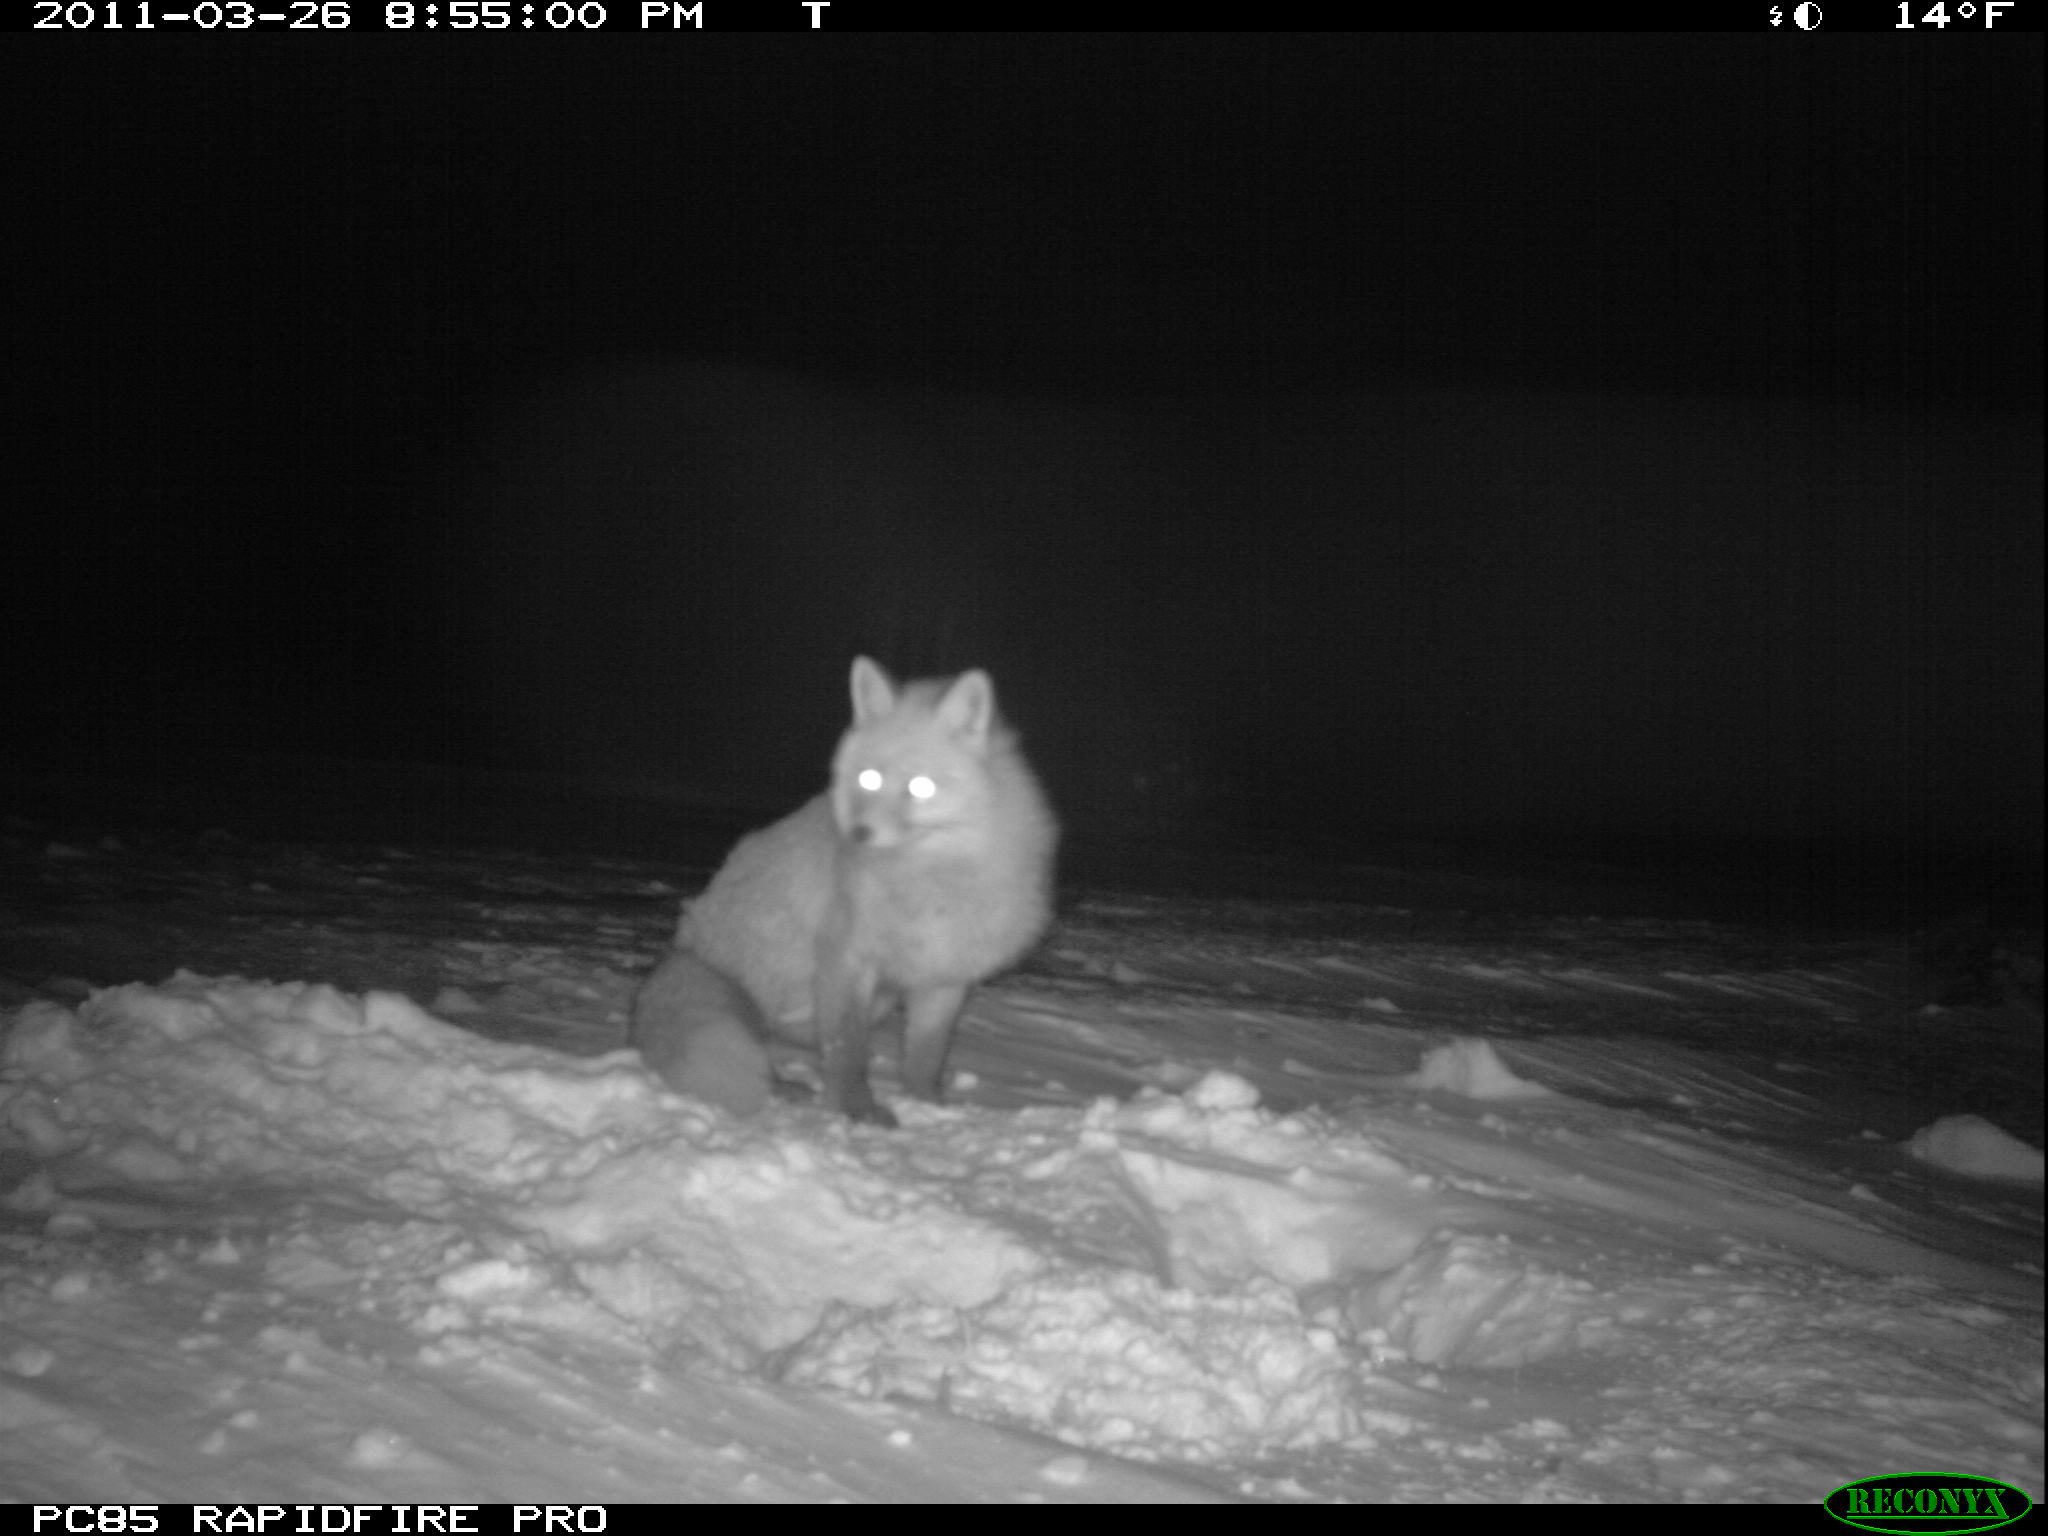
\includegraphics[width=\textwidth]{IMG_1562.JPG}
        \caption{Picture of an arctic fox at nighttime.}
    \end{subfigure}
    \caption{Images from the COAT dataset showing how a picture can contain colors or greyscale.}
    \label{fig:pictures}
\end{figure*}


\section{Dataset Directory Structure}
The pictures in the dataset is structured in directories and folders. The dataset is first divided into different years going from 2011 to 2015. Each of these folders are then again divided into the areas of the 5 camera traps in the Arctic Tundra. Inside each of these folders specified by the area, they contain folders from each site inside the specific area. Figure \ref{fig:directories} shows a cropped screenshot of the directories.

%\textbf{NOTES: (In total 1976 directories, men alle er ikke i bruk/relevant)}

\begin{figure}
\centering
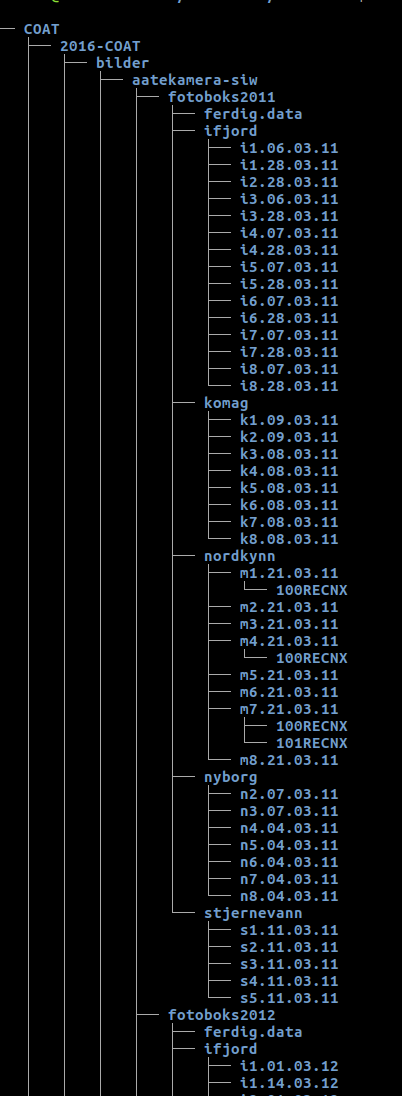
\includegraphics[scale=0.5]{directory.png}
\caption{Figure showing a cropped screenshot of the structure of the directories.}
\label{fig:directories}
\end{figure}

\section{Image Annotations}
%\textit{NOTES: Biologist and ecologists working on the COAT project have detected animals in each image and made annotations stored in excel-files containing metadata and animal classification.}

COAT provided annotations stored in excel-files with information about all of the images in the dataset that biologist and ecologists working at the COAT project have detected. The biologist have used these annotations to see what animal was present at a specific time and to see statistics. The biologist have not made these annotations for the purpose to go back in time and look at the images, which is the essential part in our approach.
The annotation contains information about a pictures location, site, date, time, animal classification, temperature in Fahrenheit, brightness, sharpness, saturation, sensitivity etc. 
 
The excel-files are structured in their own folder and each file is named as a combination of the camera traps area, it's year and the site. An example is \textit{"fotoboks2011\_nordkynn\_nordkynn.2011.xlsx"}.


The dataset contains the images metadata and animal classification, but did not contain any filenames or a filepath. We then had to find a method to find out which images correspond to the metadata in the excel-files. Fortunately, each image had metadata stored in Exchangeable Image File Format (EXIF). We recursively traverse the directories where images are located and read date-time from the metadata and store it in a new CSV-file (Comma-separated Values).
%/dictionary with date-time as key and image-path as value.
This was quite a time-consuming task because of the number of images to process.


\chapter{Architecture}
This chapter describes the architecture of the system.
The components in the system are: physical sensors, raw data, analytics and classified data, fusion of data, fused data, virtual sensors and the user interface. 
The architecture of the system is presented in Figure \ref{fig:architecture1}. The arrows indicates the dataflow between each component in the system.

%\textbf{..eller flyten av data/dataflow eller hvem som er aktiv i å gjøre akses/sende}


\begin{figure}
\centering
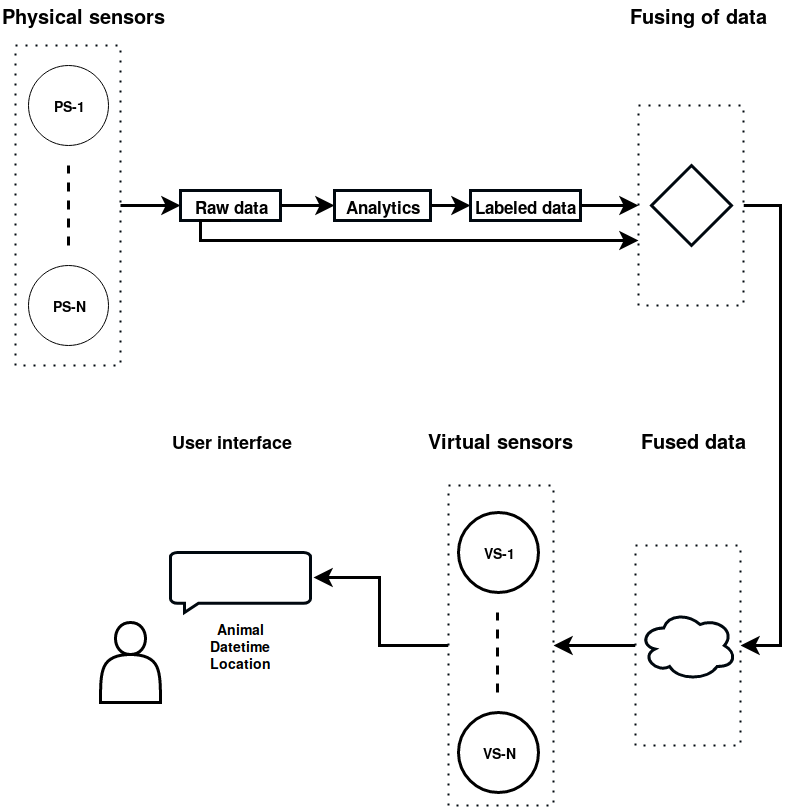
\includegraphics[width=\textwidth]{Architecture_otto5.png}
\caption{Figure showing the system architecture.}
\label{fig:architecture1}
\end{figure}


\section{Physical Sensors}
The physical sensors produce raw data. The raw data consists of images from different bait-camera sensors.
The data also contains metadata about each image, as described in Chapter \ref{chap:data_set}. 

%\textbf{Hva mer??}

\section{Raw Data, Analytics and Labeled Data}
The raw data contains images from the physical sensors and annotations in excel-files containing metadata about each image alongside labeled data, as described in Chapter \ref{chap:data_set}.

%\textbf{Hva mer??}
%\section{Analytics and Labeled Data}


%\section{Fusing of data and Fused Data}
\section{Fusing Of Data}%\subsection{Fusing of data}
Get analytics and classified data from the raw-data and annotated data.

%\textbf{Hva mer??}

\section{Fused Data}%\subsection{Fused Data}
The fused data retrieves it's data on demand. The fused data is the physical sensors location combined with necessary metadata such as date-time, location, site, year, animal classification and also how many animals there was in an image.


\section{Virtual Sensors} \label{sec:arch_vs}
The virtual sensors are divided into multiple sensors where each virtual sensor represents a different animal that scientists are interested in, like ravens, red foxes, golden eagles or polar foxes.

The virtual sensors have the same functinonalities and offers interaction between the fused data and the user interface. A user tells the user interface, described in Section \ref{sec:arch_user_int}, a task and forwards the task to the desired virtual sensor. The virtual sensor will then retrieve its results from the fused data.


%The user types in the user interface, described in Section \ref{sec:arch_user_int}, what animal he/she wants to see, where it is and the date-time and the search is redirected to the sensor related to that specific animal. The virtual sensor retrieves its result from the fused data.

%\subsection{Raven Sensor, Red Fox Sensor, Golden Eagle Sensor, no-animal sensor}
%\textit{Eller ha disse som eget kapittel "My virtual sensors".. Tror jeg utdyper mer her ettersom VS er helt like bortsett fra at de avhenger av hva slag dyr man er ute etter..}


\section{User Interface} \label{sec:arch_user_int}
A user wants to retrieve fused data about animals. The user interacts with the virtual sensor user interface. This takes care of the interaction with the virtual sensor. When a user gives a command, the desired virtual sensor retrieve data from the fused data as described in Section \ref{sec:arch_vs}, and presents the result back to the user.

%\textbf{NOTES: utdype query språk - utdype mer i design/implementation?}



\chapter{Design}
%\textbf{Client/Server, p2p, put/get, pub/sub, protokoller, FTP etc..
%BESKRIV INTERAKSJONEN MELLOM ENHETENE!!}

In this chapter we will look at the design of the system and present the design of each component of the architecture. Figure \ref{fig:design} shows the design of the system. The arrows indicates the communication lines and dataflow between each component in the system. The dotted arrows show how the data storage is structured with files and raw data.

%\ OLD
%\textit{In this chapter we will look at the design of the environment. We will present the design of the data storage, the fused data the virtual sensors and the user application. Figure \ref{fig:design} shows the design of the system. The arrows indicates the communication lines. The dotted arrows show how the data storage is structured with files and pictures.}


\begin{figure}
\centering
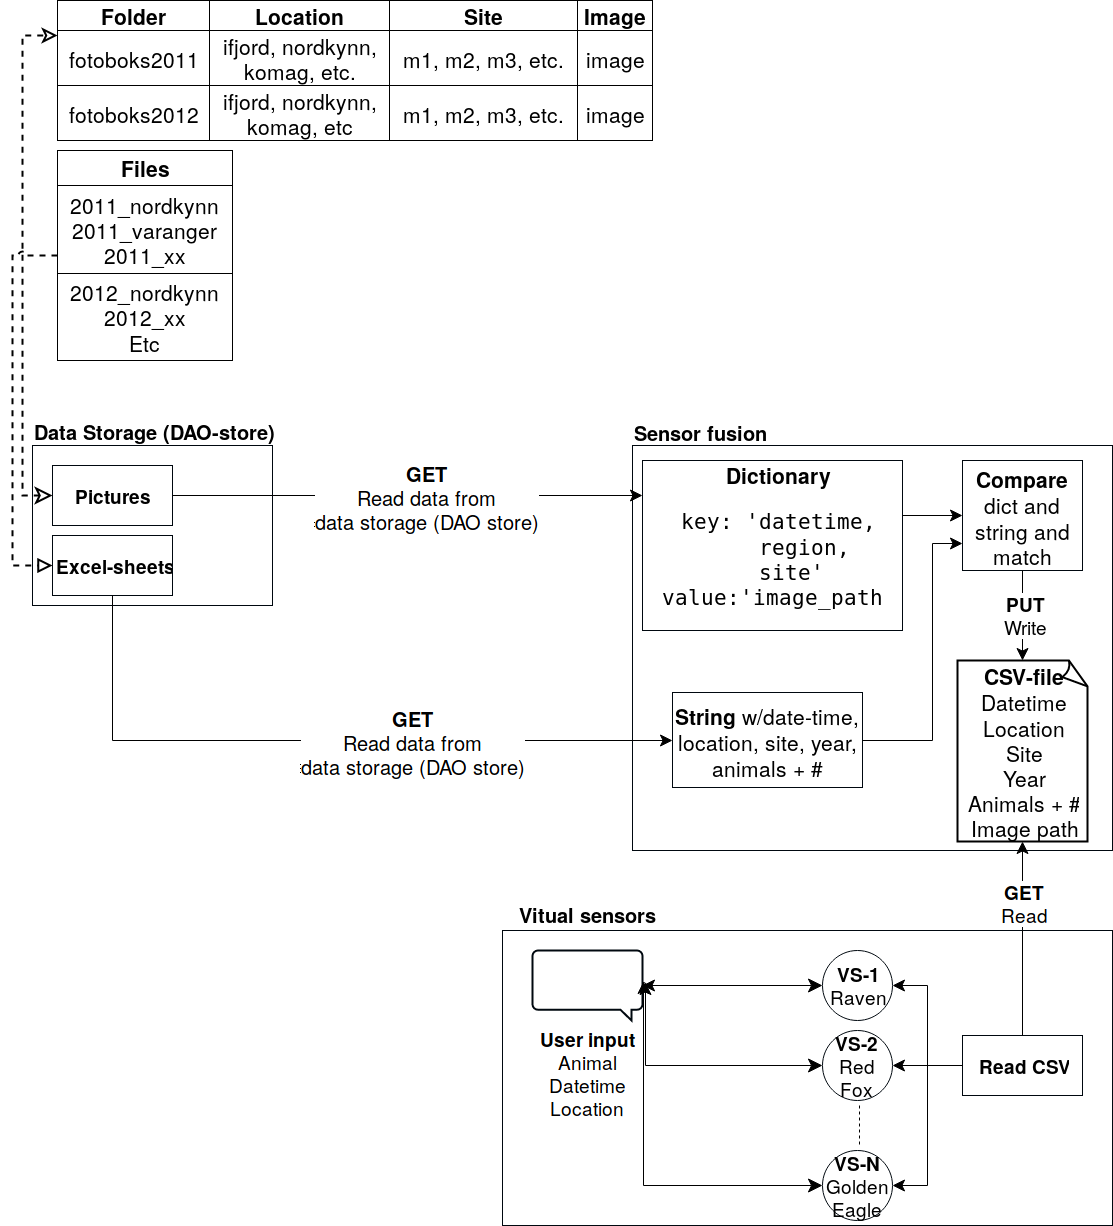
\includegraphics[width=\textwidth]{Design.png}
\caption{Figure showing the system design.}
\label{fig:design}
\end{figure}

\section{Data Storage}
%\textbf{Hvordan lagrer du data? (sensor, metadata.. Design og interface.. database, dictionary... osv}

The data storage contains raw data from the physical camera trap sensors and excel-files containing annotations for each raw data, as described in Chapter \ref{chap:data_set}.


\section{Sensor Fusion} \label{sec:des_fused}
As mentioned earlier in Chapter \ref{chap:data_set}, the dataset did not contain any filename or a filepath. It only contained image metadata such as a pictures location, date-time, site, year and animal classification. We then had to find a method to find out which images correspond to which annotation in the excel-sheet.

We recursively traverse the directories where pictures are located and read date and time from the metadata for each picture along with the annotation in the excel-sheet. The images and annotations that matched, is stored in a Python dictionary, like a key-value store, with date-time as key and image-path as value. Images and annotations that matches is stored in a new CSV-file.
As mentioned earlier, was this quite a time-consuming task because of the numbers of images to process and compare.


\section{Virtual Sensors}
%\textit{John M.: "Kan du ha flere identiske virtuelle sensorer for å prosesere i parallel? Og Er det sensorene som visualiserer, eller returnerer de data som kan  visualiseres av klienten= ut fra 4.3 høres det ut som siste"}

%\textbf{Virtual sensors probably uavhengige prosesser, ikke threads ettersom man evt vil addere flere sensorer og unnga a starte alle sensorer på nytt igjen..
%Er de virtuelle sensorene servere eller client/publisher?}

%\textbf{Otto: I design: The image(s) are displayed through an image-vision.}
%\textbf{NOTES: Divided into multiple virtual sensors depending on animal.}

\subsection{Virtual Sensors} \label{ssec:des_vs}
The virtual sensors are divided into multiple sensors depending on animals. The respective virtual sensor must handle events from the user. Assume a user wants to find pictures of a red fox at a specific time.  The user interface makes the respective virtual sensor aware of the task. The virtual sensor will then go to a list of all red foxes that are located from the fused data and search for the specific request. If the virtual sensor find pictures that are similar to the request from the user, one and one picture is visualized on the computer screen to the user.

The virtual sensors in this approach are functions in a sequential system. They could have been threads in a parallel program or the best solution would be if the virtual sensors where independent subprocesses because that would not affected other virtual sensors when a virtual sensor is added or removed from the system, as well as if one virtual sensor crashes. \textit{Note: Er dette mer diskusjonsmateriale? Eller ha det med her også?}


%\subsubsection{Raven Sensor}
%\subsubsection{Golden Eagle Sensor}
%\subsubsection{Red Fox Sensor}

\subsection{User Application} \label{ssec:des_user}
The user-application is the connection between the user and the virtual sensors. It gets input from the user and sends a request to the virtual sensor based on its input. The user-applications goal is to make an interface that is easy to use and to show images that the user want to see. The main menu is shown in Listing \ref{lst:mainmenu}.
The user only need to specify the following 3 parameters for the virtual sensor:

\begin{itemize}
\item \textbf{Animal:} The user can choose to see 3 different animals; raven, red fox and the golden eagle. The user can also chose to see pictures with no animals in it. The reason that the user only can chose between these 4 categories is that these are the only virtual sensors that are implemented in this version of the system.

\item \textbf{Date-time:} If the user wants a specific date-time the picture(s) was taken, he/she can specify the date and time in this section. If the user leave this field blank, all dates will included when the system search for pictures.

\item \textbf{Location:} At last, the user can chose if he/she wants the picture to be located anywhere specific. The only valid arguments in this field is Nordkynn, Komag, Nyborg or Stjernevann since these are the only names in the CSV-file in the fused data.
\end{itemize}

\begin{lstlisting}[frame=single,caption={Main menu },label={lst:mainmenu}, language=Python]

**** WELCOME! ****
******************

Write what you want to see
(Raven, RedFox, GoldenEagle): 

Write when you want to see (blank is all dates): 
E.g: 2011:03:24 or 2011:04:24 10:10:00

Where do you want the animal to be located
(nordkynn, varanger: komag, nyborg, stjernevann):
\end{lstlisting}



\iffalse 
\begin{table}
\centering
\begin{tabular}{|l|l|}
\hline
Content left & Content right\\
\hline
\end{tabular}
\caption{A table}
\end{table}
%\newpage
\begin{lstlisting}[frame=single,caption={Small C program},language=C]
#include "stdio.h"
#define e 3
#define g (e/e)
#define h ((g+e)/2)
#define f (e-g-h)
#define j (e*e-g)
#define k (j-h)
#define l(x) tab2[x]/h
#define m(n,a) ((n&(a))==(a))

long tab1[]={ 989L,5L,26L,0L,88319L,123L,0L,9367L };
int tab2[]={ 4,6,10,14,22,26,34,38,46,58,62,74,82,86 };

main(m1,s) char *s; {
  int a,b,c,d,o[k],n=(int)s;
  if(m1==1){ char b[2*j+f-g]; main(l(h+e)+h+e,b);
    printf(b); }
  else switch(m1-=h){
    case f:
      a=(b=(c=(d=g)<<g)<<g)<<g;
      return(m(n,a|c)|m(n,b)|m(n,a|d)|m(n,c|d));
    case h:
      for(a=f;a<j;++a)
        if(tab1[a]&&!(tab1[a]%((long)l(n))))
          return(a);
    case g:
      if(n<h)return(g);
      if(n<j){n-=g;c='D';o[f]=h;o[g]=f;}
      else{c='\r'-'\b';n-=j-g;o[f]=o[g]=g;}
      if((b=n)>=e)
        for(b=g<<g;b<n;++b)o[b]=o[b-h]+o[b-g]+c;
      return(o[b-g]%n+k-h);
    default:
      if(m1-=e) main(m1-g+e+h,s+g); else *(s+g)=f;
      for(*s=a=f;a<e;) *s=(*s<<e)|main(h+a++,
      (char *)m1);

    }
}
\end{lstlisting}
\fi



\chapter{Implementation}
\section{Overview}
%\textbf{Threads, data structures, language...}
This chapter will elaborate on how we implemented the system, general implementation requirements, issues and choices. 
%In the rest of this chapter 
We will first look at some libraries used in this implementation, then we will take a look at the data storage in Section \ref{sec:imp_storage} and the sensor fusion in Section \ref{sec:imp_senfus}. At last, we will describe the virtual sensors and the user application in Section \ref{sec:imp_virsens}.

The system is implemented and written in the high-level programming language Python 2.7\footnote{\url{https://www.python.org/}}. This was a practical choice because we were familiar with it from previous projects, it is an object oriented language and if offers multiple different libraries. The libraries used in this implementation are mentioned below.
%We made this choice because Python is object oriented and it offers different frameworks that are relevant for this implementation.


\subsubsection{Exchangeable Image File Format - EXIF} \label{sssec:imp_exif}
%\ac{EXIF}
Exchangeable Image File Format (EXIF) is a standard that specifies the formats for images, sound, scanners and other systems recorded by digital cameras. This standard consists of image information of the EXIF image file or the EXIF audio file.

Python have a module called  EXIF 2.1.2\footnote{\url{https://pypi.python.org/pypi/ExifRead}}, to extract the metadata(image information from the jpg-files.

\subsubsection{Pandas Dataframe} \label{sssec:imp_df}
Pandas\footnote{\url{http://pandas.pydata.org/}} is an open source Python Data Analysis Library which provides high-performance and easy-to-use data structures. It is a NUMFocus\footnote{\url{https://www.numfocus.org/open-source-projects/}} sponsored project which will help ensure success of the development of pandas as a open-source project in world class. A dataframe\footnote{\url{https://pandas.pydata.org/pandas-docs/stable/generated/pandas.DataFrame.html}} is a two-dimensional, dynamic tabular data structure with labeled axes (rows and columns), just like an excel-file.

\subsubsection{OpenCV} \label{sssec:imp_cv}
OpenCV V2.4.9.1\footnote{\url{https://opencv-python-tutroals.readthedocs.io/en/latest/}} is an open-source library which provides the functionality for loading and preprocessing images.

%OpenCV was started at Intel in 1999 by Gary Bradsky and it was released in 2000. OpenCV supports many algorithms related to Machine Learning and Computer Vision. 
%At this time, OpenCV supports a wide range of programming languages such as C++, Python and Java and is also available on different platforms like Windows, Linux, OS X etc. OpenCV-Python combines the best qualities of OpenCV C++ API and Python language.%


\section{Data Storage} \label{sec:imp_storage}
The data storage contains raw data and prepossessed images that are structured and sorted by animals. Unfortunately, these preprossesed images don't consists of any image metadata so we don't have any information of when the image is taken. Therefore, the solution is to traverse the whole data storage and find the raw data with metadata and compare these to the excel-files containing information like date, time, location and site.
%\textbf{HOW DID I TRAVERSE}


\section{Sensor Fusion} \label{sec:imp_senfus}
\subsection{Raw Data Information Extraction} \label{ssec:imp_rawdata}
The raw data in the data storage is traversed by walking the OS directories. If the traversed file ends with JPG, the image information in the EXIF is being extracted and the datetime value is read. This datetime along with the images site, region and image path is stored in a Python dictionary, where the datetime, site and region is key and the image path is the value. This was as mentioned earlier, a time-consuming task because of the 1.6 millions of pictures that was being processed.

During implementation we came across a problem with the folders containing white-space and UTF-8 character. An example of a folder is \textit{'/../Bilder til institutt for informatikk/åtekamera (Siw)'}. 
%This makes it difficult to extract images due to the reason that the new CSV-file had white-space between each characters.
%This is described further in Section \ref{ssec:imp_compare}. 

This was an obstacle during implementation because it led to difficulties reading the folder-names when they contained characters the system wouldn't interpret. The solution was to change the folder-names manually and avoid the use of whitespace and UTF-8 characters. An example of a new folder is \textit{'../bilder/aatekamera-siw'}.

%\textbf{NOTES: folder-path inneholdt mellomrom og æøå, gjorde det vanskelig å hente ut bilder når pathen krøllet seg... brukte litt tid på å prøve meg fram, endte med å snakke med JM om å endre folder-navn uten mellomrom og æøå.. Snakke om det i compare når jeg leser fra csv-filen ettersom det er i csv-filen det bugger seg når jeg skal lese ut path når den inneholder space og æøå?}

%As described in Section \ref{ssec:imp_rawdata}, the folder-names contained white-spaces and UTF-8 characters. This was an obstacle during implementation because it led to difficulties reading the folder-names when they contained characters the system wouldn't interpret. The solution was to change the folder-names manually and avoid the use of whitespace and UTF-8 characters.

%/home/camilla/Documents/daoshare2/COAT/2016-COAT/bilder/aatekamera-siw
%'/home/camilla/Documents/daoshare/COAT/camtraps/COAT/fra-COAT/Bilder til institutt for informatikk/åtekamera (Siw)'


\subsection{Excel files Extraction} \label{ssec:imp_excel}
The excel files contains annotations for each image. To read excel files, we use Pandas Dataframe, described in Section \ref{sssec:imp_df}. From the excel files, we extract information like date, time, animals, region, site and year. The necessary information about each animal is stored in a string.

During implementation we came across a problem with inconsistency between cells in the same row. The problem was that the datetime cells information was inconsistent with the information in cells day, month, year, hours and minutes, shown in Figure \ref{fig:inconsistency}. Our solution was to alter and concatenate the correct values to make a new datetime.

\begin{figure}[b]
\centering
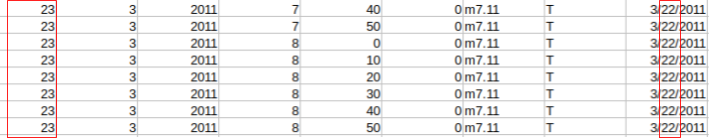
\includegraphics[width=\textwidth]{inconsistency2.png}
\caption{Shows inconsistency between cells in rows in excel file.}
\label{fig:inconsistency}
\end{figure}

%\textbf{NOTES: Solution: overwrite moth to month? Not done, though about it while writing this now... Only tried with two excel files that contains "moth", time restrictions and wanted to find some pictures instead of nothing}

Another problem was that the cells containing column-names was different. One example is that month was written \textit{"moth"} in some excel files and \textit{"month"} in others. Because of time constraints, we only used the excel files containing the word "moth" since this was the first excel-file to be extracted and our intent was to get images to visualize. 

A different problem was that some column-header names was written with a big letter like \textit{"Time"} in some excel files and other contained \textit{"time"}. Our solution was to make every column header into lowercases using Pandas Dataframe function, \textit{pandas.Series.str.lower()}.


%\textbf{NOTES: ..Excel-file har også æøå som ikke vises i Ubuntu sin excel libre offie calc.. Kanskje bare hos meg, men burde gått igjennom og hatt en consistency mellom navn.. Biologer brukte Windows, jeg Ubuntu.. kanskje noe rot der.. men burde egentlig fikse på raw data uansett?}

One more problem arose when some of the excel-file contained table-headers with UTF-8 characters, as seen in Figure \ref{fig:utf8}. These characters won't be interpreted by the system and the table-headers will not be readable.


\begin{figure}[b]
\centering
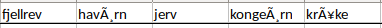
\includegraphics[width=\textwidth]{utf8.png}
\caption{Shows table-headers with unsupported UTF-8.}
\label{fig:utf8}
\end{figure}

\subsection{Comparison of data} \label{ssec:imp_compare}
%\textit{Disse sammenlignes og de som matcher blir skrevet til en ny CSV fil med nødvendig info for å finne bilde. Samlet både metadata og annotations fra excel fil så kan de sammenlignes.. 
%Tar lang tid, mange bilder og mange rows i excel.. det som bruker mest tid..}


The extracted metadata from the images and the annotations in the excel files that matches, is stored in a CSV-file (Comma-separated Values). We chose to store the fused data in a new CSV-file because of the large number of images to process. It will simplify search in the future since it will be faster to search through the fused data in the CSV instead of searching through the raw data and compare them with the annotations. This is not the best choice, however it is a introduction to a solution.

%\textbf{NOTES: Why stored in a new CSV-file? begin somewhere, simplify search next time.. no database.. because of number of images to process - takes time, solution is to make a csv-file to store aggregated data so we don't need to search through the whole data storage next time, but only the new csv file.. not optimal or best solution, but works and it's a start..}


\section{Virtual Sensors} \label{sec:imp_virsens}
\subsection{Virtual Sensors} %\label{ssec:imp_vsensor}
%\textit{ikke threads ettersom man evt vil addere flere sensorer og unnga a starte alle sensorer på nytt igjen..
%Er de virtuelle sensorene servere eller client/publisher?}

The virtual sensors are implemented as functions, not threads or independent subprocesses, as mentioned in Section \ref{ssec:des_vs}. The reason for this choice is because we needed somewhere to start and this was the ... \textbf{..start somewhere and eventually lack of time/time constraints and wanted to show something instead of nothing..}


%\textbf{NOTES: Valgte å fokusere på tre dyr (og alle dyr/bilder eller ingen dyr i bilde) ettersom de var de som det var flest av i excel-arkene.. and time constraints.. ville ha noe å vise enn ingenting} \\
%\textbf{Write about that you don't have all animals, only the ones who is most of in csv-file, not every animal is presented in the dataset..}

We also chose to focus on virtual sensors for three different animals and images without any animals in it. The three animals were the red fox, ravens and the golden eagle. We made this choice because these were the animals that were \textbf{most present/appeared the most} in the annotations in the excel files that were extracted.


%\textit{NOTES: John M.: "Kanskje bare gjøre et poeng at dette bare ble valgt på grunn av kjennskap til det / bruk i andre prosjekter og at nøyaktig hvilket verktøy som brukes til visualisering ikke var fokus."}

The OpenCV library is used to visualize images to the user. The library read the images it is given and display these on the screen to the user. The reason for choosing this visualization library was because of experience with this in previous projects and also that our focus was not primarily on which library to use when visualizing images.



\subsection{User application} \label{ssec:user}
The user application is implemented as an interface in the terminal that communicates with the virtual sensors.

There is currently not possible for more than one user to be connected in the same application at a time. Because of lack of time, we have not thought about implementing this. Our focus has been making a prototype of the user interface to be easy to use for biologists/users and to show images on the users request.


\chapter{Evaluation} \label{chap:evaluation}
This chapter describes the experimental setup and metrics used to evaluate the implemented system. 

%metrics, define (CPU, memory, latency.), benchmarks (micro, kernel...
%How to measure, where done, PSEUDOCODE

\iffalse
\ NOTATER:
%\begin{itemize}
%\item python -m cProfile -s cumtime find_folder_ok_concurrent.py 

\item Time: \\
Finding folders and metadata takes:  1:43:13.488799 (103,2167 minutes), \\
Reading excel file takes:  0:00:17.413845 (0.2833 minutes),\\
Comparing takes:  4:43:30.705587 (283.5 minutes),\\
Overall time is  6:27:01.608355 (387.0167 minutes).\\
Med alle bilder m/metadata og \\
hele fotoboks2011\_nordkynn\_nordkynn.2011.xlsx.

\item New time: \\
Finding folders and metadata takes:  1:46:17.406581(= 106.2833 minutes) \\
Reading excel file takes:  0:01:07.686779 (= 1.1167 minutes) \\
Comparing takes:  19:03:11.177869 (= 1143.1833 minutes) \\
Overall time is  20:50:36.271415 (= 1250.6 minutes) \\
Med alle bilder m/mETADATA og hele nordkynn og varanger

\item "Concurrent" python find\_folder\_ok\_concurrent.py \\
Finding folders and metadata takes:  1:30:50.250732 (= 90.8333 minutes) \\
Reading excel file takes:  0:00:18.127597 (= 0.3 minutes)\\
Comparing takes:  4:18:33.368199 (= 258.55 minutes)\\
Overall time is  5:49:41.746759 (= 349.6833 minutes)\\
-- Pool(processes=4) \\
FRA fotoboks2011\_nordkynn\_nordkynn.2011.xlsx

\item "Concurrent" igjen \\
Finding folders and metadata takes:  1:44:18.788013 (= 104.3 minutes)\\
Reading excel file takes:  0:00:17.269817 (= 0.2833 minutes)\\
Comparing takes:  3:54:23.483186 (= 234.3833 minutes)\\
Overall time is  5:38:59.541248 (= 338.9833 minutes)\\
-- Pool(processes=100)\\
FRA fotoboks2011\_nordkynn\_nordkynn.2011.xlsx

\end{itemize}
\fi

\section{Experimental Setup}
All experiements were done on a Lenovo ThinkCenter with an Intel® Core™ i5-6400T CPU @ 2.20GHz × 4, Intel® HD Graphics 530 (Skylake GT2), 15,6 GiB memory and 503 GB disk. It ran on Ubuntu 17.04 64-bit with gcc V6.3.0 compiler and Python V2.7.13.

\section{Experimental Design}
%\textbf{Measured time when executed in all 4 experiments.. Hadde en test med nordkynn, en med nordkynn og varanger, og 2 tester hvorav den ene var nordkynn med 4 prosesser (concurrent) og den andre var nordkynn med 100 prosesser (for concurrent compare). Python process pool (multiprocessing: multiprocessing is a package that supports spawning processes using an API similar to the threading module). Prøvde også med over 500 processer, men ga ikke noe bedre resultat.. Tror det blir mye overhead..}

We decided to measure execution time on the five different experiments. We measured execution time on the new csv-file that contained only fused data from Varanger and the new CSV-file that contained fused data from Varanger and Nordkynn. We also ran three experiments where we tried to run the comparison between images and annotations concurrently with 4, 100 and 500 processes by using a multiprocessing library in Python that supports spawning processes using an API similar to the threading module.

\section{Results}
In this section we will discuss the results of the testing described in the sections above...

What does the result say?
Each experiment, result, meaning

\subsection{Measure Execution Time}
\textbf{Most time during finding folder and read metadata and comparing.. Read excel file is faaaast!!}

%followed/pursued

Figure \ref{fig:time_chart500} shows the time to execute different parts of the system. We can see that the comparison between images and annotations is the part of the system that takes the longest time followed by the part that finds folders and read metadata from the raw data. This is because of the of the high number of data to process

The only bar in Figure \ref{fig:time_chart500} that stands out/emerge? from the other, is the time used when comparing data from both Varanger and Nordkynn.

\iffalse
%\begin{figure}
\centering
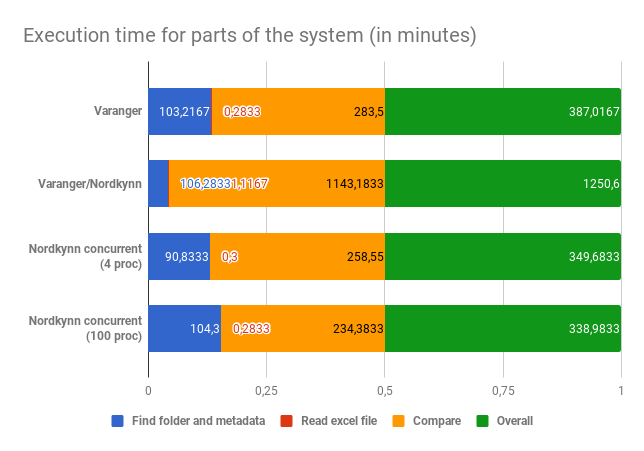
\includegraphics[width=\textwidth]{chart.png}
\caption{Figure showing time to execute different parts of the system (in minutes).}
\label{fig:time_chart}
\end{figure}
\fi

\iffalse
%\begin{figure}
\centering
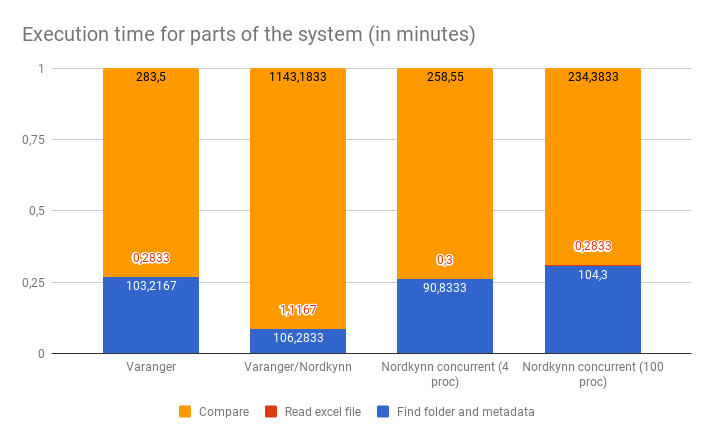
\includegraphics[width=\textwidth]{chart2.png}
\caption{Figure showing time to execute different parts of the system (in minutes).}
\label{fig:time_chart2}
\end{figure}
\fi

\begin{figure}
\centering
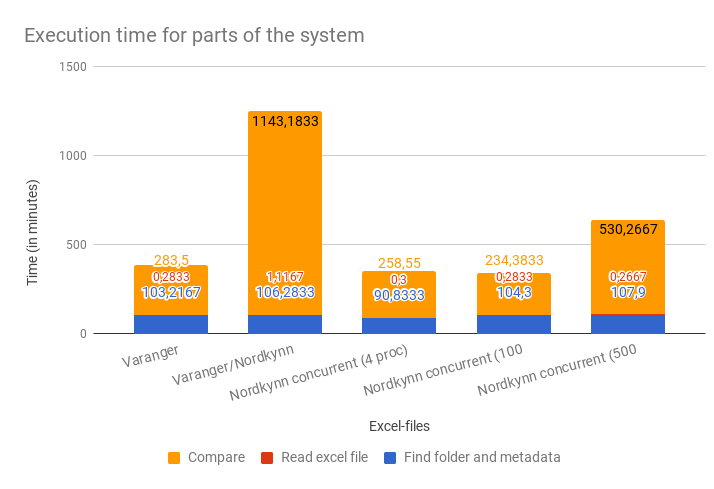
\includegraphics[width=\textwidth]{chart500proc_new.png}
\caption{Figure showing time to execute the system (in minutes).}
\label{fig:time_chart500}
\end{figure}

\textbf{When only Varanger, same time for sequential" and concurrent.. Eneste som skiller seg ut er Varanger og Nordkynn sammen, men ikke så rart ettersom det er fra 2 lokasjoner og ikke en som de andre.. Mer data å sammenligne. Concurrent med 500 processer skiller seg også litt ut i forhold til de andre concurrent, men tror dette har med overhead eller noe å gjøre..}

Figure \ref{fig:time_chart_overall} show the time for the whole system to run. As we can see, ...

\begin{figure}
\centering
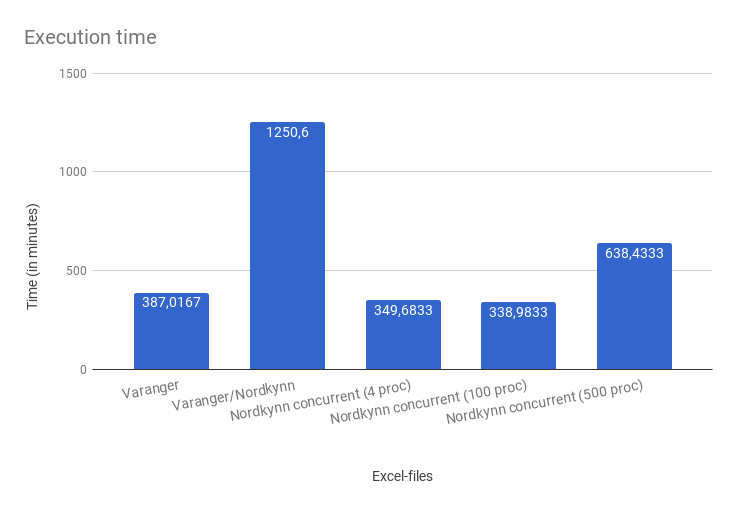
\includegraphics[width=\textwidth]{chart3_new.png}
\caption{Figure showing time to execute the system (in minutes).}
\label{fig:time_chart_overall}
\end{figure}

\iffalse
%\begin{figure}
\centering
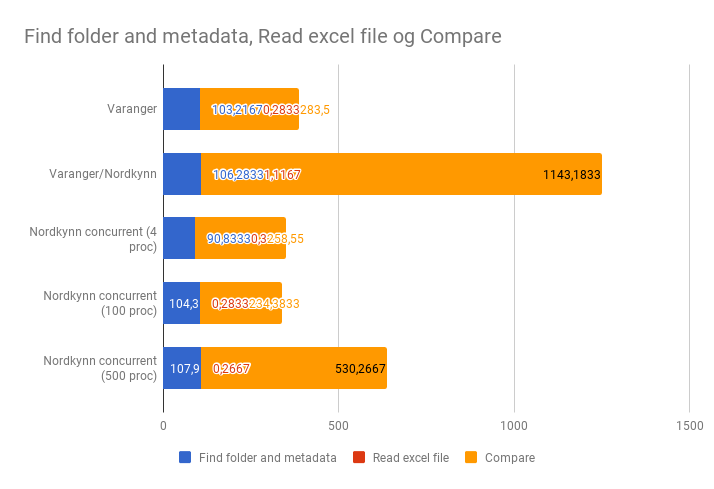
\includegraphics[width=\textwidth]{chart_500proc_new.png}
\caption{Figure showing time to execute the system (in minutes).}
\label{fig:time_chart500new}
\end{figure}
\fi


\subsection{Measure CPU}
Doing the experiments now..

\subsection{Measure Memory}
Doing the experiments now..

\subsection{Disk Read/Write}
Doing the experiments now..




\chapter{Discussion}
%Idea, architecture, design, results, other solutions, "arch have scale-problem?".

%\begin{itemize}
%\item Virtual sensors probably uavhengige prosesser, ikke threads ettersom man evt vil addere flere sensorer og unnga a starte alle sensorer på nytt igjen.. HVORFOR valgte jeg løsningen som jeg gjorde, og er dette er andre løsninger..
%\item Burde lage egne gorutiner/subprocesser/classer for hvert dyr. alle er en basic class med f. eks ID, TYPE, CAPABILITIES, HISTORIKK?, QUERIES/RAW DATA..
%\item Kombinere VS søke på "ravn \& rev eller ravn | rev.. mellom 2 tidspunkt, nordkynn | varanger... etc..
%!!!!!!!!!!!!\item hash-map instead of multiple lists with different animals. hash on animal and/or place
%\item parallel/concurrent program when doing metadata-collecting and reading from excel-files and writing to csv. Python - bad experience with threads/subprocess, golang probably better?
%\item Drawback with Python - not that good at threading/parallel/concurrency.. Python is not good for multi-processor/multi-core work. Prøvde å bruke multiprocess-bibliotek med pools med processer.. Ble litt bedre, men ikke noe spesielt.. Golang ville kanskje vært bedre mtp concurrency. Gjør GOlang when performance is critical..
%\item Forskjellig språk har focus på forskjellig ting og er gode forskjellige ting.. Uansett hvilket språk man velger pga en fordel, vil det mest sannsnylig være et annet språk som er bedre på en annenn ting du skal implementere.. som f. eks. Golang bedre concurrent enn Python..
%\item Updates of "database" in background, not on demand -> future work?
%\item Et script som går gjennom alle excel-filene som den ikke har lest og lagrer data eller noe sånt.. Bør gjøres i bakgrunnen/ikke on-demand. Filer som slutter på .xlsx leses og evt. legges i en liste som kan sjekke senere om filen er blitt lest eller ikke..
%\item Brukte mye tid på data behandlingen og datasettet.. mye tull med utf-8 og whitespace osv, og forskjellige datoer i excel-fil..
%\item Og mye tid på excel-fil som inneholdt forskjellige datoer etc. som gjorde at jeg måtte trikse og mikse for å få riktig dato så jeg fikk opp riktig bildet/få opp bildet i det hele tatt..
%\end{itemize}

%some of the points where we met problems
This chapter discusses our approach, experience and why we chose the solution we ended up with...

\section{Virtual Sensors}
As mentioned in previous chapters, are the virtual sensors functions in our approach. We choose this approach because of we firstly wanted to find images from the fused data and show them to the users. Another reason is because of time limitations.

Another solution to this approach of virtual sensors is to implement them as threads. This would again not be the best solution if for example the system should be able to add more virtual sensors during run-time. To solve this problem, we could have implemented the virtual sensors as independent processes which would not be affected when another virtual sensors is added, removed or at worst crash/fail.

A virtual sensor could also be implemented as an abstraction or a general class with parameters such as \textit{id, type, capabilities, history and queries or raw data}. This parameters will then say something about what kind of virtual sensor it is, what it can do (show images, find new data if any etc.) and support for queries from user.

\iffalse
\begin{itemize}
\item Id
\item Type
\item Capabilities
\item History
\item Queries or raw data
\end{itemize}
\fi

\section{Queries}
Our approach support queries with only one option per animal, location and datetime, described in Section \ref{ssec:des_user}. The reason for this choice is because we started with a simple implementation with intent to expand at a later point. The first implementation only contained what kind of animal the user wanted to see. At later point, both location and datetime was added to narrow the search result. Due to time constraints, we didn't have time to implement more advanced search functionalities.

An improvement would then be to support operations like AND and OR for all three options in the user interface.
Then the user could for example search for \textit{"fox || raven"}, \textit{"fox \&\& raven"}, \textit{"Nordkynn || Stjernevann"} or to choose an interval between two datetimes like \textit{"26-04-2016 - 30-04-2016"}. This would make image search more flexible and add more advanced search queries for the users.
%This would open the possibility for a combination/fusing of different virtual sensors...

\section{Sequential vs. concurrent implementation??}
%Use a language more suitable for performance (execution time), like Golang..
As described in Chapter \ref{chap:evaluation}, the execution time of system is not satisfying (or something...). Using Pythons multiprocessing library did not solve any problem with time spent on comparing images and annotations. The reason we tried Pythons multiprocessing library was to see if it made any performance-improvement on execution time compared to the sequential system. If it haven't been for the time constraints, we would try to implement another solution with threads.

Another solution is to change the language from Python to The Go Programming Language\footnote{\url{https://golang.org/}}. One of Go's strongest sides is a built-in concurrency based on CSP \cite{hoare}. Go is built with concurrency in mind and has goroutines instead of threads. Another advantages of goroutines is that it comes with a built-in primitive to communicate between themselves by using something called channels. There is also no need for some kind of mutex locking when sharing data structures compared to threads.


\section{On-demand vs. background "updates" from datastorage}
%Search server for new radar measurements in. If new data found, send to radar rainfall estimator.. \cite{hill}.
Current solution does not support the ability to traverse the data storage with multiple excel-files. It only takes one and one excel-files that is predefined and extracts it's data.

A quick fix to this problem is to traverse the directory where the files are located and then check if the files ends with \textit{".xlsx"}. These files will then be extracted and stored in for example a Pandas Dataframe like the current approach. The file-names could also be stored in the system to prevent to read the same files again if any new files is stored in the data storage.

We did not choose this approach because the comparing of images and annotations is a time-consuming task where one file took several hours and comparing with two excel-files took over 20 hours as described in Chapter \ref{chap:evaluation}. %scale problem - kan man si det??

Another challenge with this approach is that some data in the excel-files contains characters with UTF-8 encoding. The challenge is then to interpret the data, described in Section \ref{ssec:imp_excel}.

%A solution would be to search the data storage for new information and if new data is found, send it to the fusion of data


%Brukte mye tid på data behandlingen og datasettet.. mye tull med utf-8 og whitespace osv, og forskjellige datoer i excel-fil..

%Og mye tid på excel-fil som inneholdt forskjellige datoer etc. som gjorde at jeg måtte trikse og mikse for å få riktig dato så jeg fikk opp riktig bildet/få opp bildet i det hele tatt..

\chapter{Conclusion}
\textbf{NOTES: Focus on showing an image to user, spent lot of time with dataset and modify so data could be extracted, many improvements - also described in future work.. Experiment show need for concurrent system, a lot of data/big data to process}

In this project, we have implemented a system...

Our experiments showed that ...

\section{Contributions?}
Har denne i introen også..

\chapter{Future Work}
\begin{itemize}
\item Concurrent lesing av excel-filer (alle sammen). Lesing går egentlig greit, men burde hatt en løsning som leste alle filer som sluttet på .xsls eller noe lignende og så evt legge navne til filene i en liste slik at man kan sjekke om det filen er lest fra før av hvis man legger til nye filer i data storage..
\item Concurrent lesing av metadata og traversering
\item Concurrent sammneligning!!!
\item VS er subproseser/channels(?) i GO slik at man evt kan fjerne/legge til sensorer om man vil
\item Gjøre i Golang?
\item Concurrent VS: kan hente data fra flere sensorer eller kombinere flere VS.. Eks: ravn \& rev eller ravn | rev.
\item Query for å hente bilder mellom 2 tidspunkt
\item Oppdatere/sjekek frequent, ikke som nå (on-demand).
\end{itemize}


\chapter{Appendix?}
readme, source code, dataset measurement RAW
\backmatter


%%% BIBLOGRAPHY

\newpage{}

\begin{thebibliography}{9}
%1
\bibitem{VirtualSensors2006}
S. Kabadayi and A. Pridgen and C. Julien,
\newblock {\em Virtual Sensors: Abstracting Data from Physical Sensors}, 2006,
\newblock in {\em 2006 International Symposium on a World of Wireless, Mobile and Multimedia Networks(WoWMoM'06), 6 pp.-592}.

%2
\bibitem{Ciciriello}
Ciciriello, Pietro and Mottola, Luca and Picco, Gian Pietro,
\newblock {\em Building Virtual Sensors and Actuators over Logical Neighborhoods}, 2006,
\newblock in {ACM, 19--24}.
\newblock {\em \url{http://doi.acm.org/10.1145/1176866.1176870}}.

%3
\bibitem{TinyOS}
Hill, Jason and Szewczyk, Robert and Woo, Alec and Hollar, Seth and Culler, David and Pister, Kristofer,
\newblock {\em System Architecture Directions for Networked Sensors}, 2000,
\newblock in {\em  ASPLOS-IX: Proc. of the 9 nt Int. Conf. on
Architectural Support for Programming Languages and
Operating Systems}, pages 93–104.

%4
\bibitem{Mottola2006}
Mottola, Luca and Picco, Gian Pietro,
\newblock {\em Logical Neighborhoods: A Programming Abstraction for Wireless Sensor Networks}, 2006,
\newblock in {\em  Distributed Computing in Sensor Systems: Second IEEE International Conference, DCOSS 2006, San Francisco, CA, USA, June 18-20, 2006. Proceedings}, pages 150--168.
\newblock {\em \url{https://doi.org/10.1007/11776178_10}}.

%5
\bibitem{Mottola2006_2}
Mottola, Luca and Picco, Gian Pietro,
\newblock {\em Programming Wireless Sensor Networks with Logical Neighborhoods}, 2006,
\newblock in {\em  Proceedings of the First International Conference on Integrated Internet Ad Hoc and Sensor Networks},
 series = {InterSense '06}, pages 150--168.
\newblock {\em \url{http://doi.acm.org/10.1145/1142680.1142691}}.

%6
\bibitem{tinyDB}
Madden, Samuel R. and Franklin, Michael J. and Hellerstein, Joseph M. and Hong, Wei,
\newblock {\em TinyDB: An Acquisitional Query Processing System for Sensor Networks}, March 2005,
\newblock in {\em  ACM Trans. Database Syst. Vol. 30, Nr. 1}, pages 122--173.
\newblock {\em \url{http://doi.acm.org/10.1145/1061318.1061322}}.

%7
\bibitem{cougar}
Yao, Yong and Gehrke, Johannes,
\newblock {\em The Cougar Approach to In-network Query Processing in Sensor Networks}, September 2002,
\newblock in {\em  SIGMOD Rec., Vol. 31, Nr. 3}, pages 9--18.
\newblock {\em \url{http://doi.acm.org/10.1145/601858.601861}}.

%8
\bibitem{hill}
David J. Hill and Yong Liu and Luigi Marini and Rob Kooper and Alejandro Rodriguez and Joe Futrelle and Barbara S. Minsker and James Myers and Terry McLaren,
\newblock {\em A virtual sensor system for user-generated, real-time environmental data products}, 2011,
\newblock in {\em  Environmental Modelling \& Software, Vol. 26, Nr. 12}, pages 1710 - 1724.
\newblock {\em \url{http://www.sciencedirect.com/science/article/pii/S1364815211001988}}.

%9
\bibitem{coatplan2016}
Ims, R.A., Jepsen, J.U., Stien, A. \& Yoccoz, N.G. 2013,
\newblock {\em Science plan for COAT: Climate-ecological Observatory for Arctic Tundra. Fram Centre Report Series 1}, 2013,
\newblock in {\em  Fram Centre, Norway, 177 pages.}
\newblock {\em \url{http://www.framsenteret.no/getfile.php/2435814.1574.xyxruwywpp/FinalPDF_COAT.pdf}}.

%10
\bibitem{coat2016}
Åshild Ø. Pedersen, A. Stien, E. Soininen, and R. A. Ims,
\newblock {\em Climate-ecological observatory for arctic tundra-status 2016}, Mars 2016,
\newblock in {\em  Fram Forum 2016, pages 36-43.}
%\newblock {\em \url{http://www.framsenteret.no/getfile.php/2435814.1574.xyxruwywpp/FinalPDF_COAT.pdf}}.

%11
\bibitem{methodseco}
S. Hamel, S. T. Killengreen, J.-A. Henden, N. E. Eide, L. Roed-Eriksen, R. A. Ims, and N. G. Yoccoz,
\newblock {\em “Towards good practice guidance in using camera-traps in ecology: influence of sampling design on validity of ecological inferences}, 2013,
\newblock in {\em Methods in Ecology and Evolution, vol. 4, no. 2. pp. 105-113}
%\newblock {\em \url{http://www.framsenteret.no/getfile.php/2435814.1574.xyxruwywpp/FinalPDF_COAT.pdf}}.

%12
\bibitem{dice}
Gun\u{a}, \c{S}tefan and Mottola, Luca and Picco, Gian Pietro,
\newblock {\em DICE: Monitoring Global Invariants with Wireless Sensor Networks}, June 2014,
\newblock in {\em ACM, vol. 10, no. 4. pp. 54:1--54:34}
\newblock {\em \url{http://doi.acm.org/10.1145/2509434}}.

%13
\bibitem{hoare}
Hoare, C. A. R.,
\newblock {\em Communicating Sequential Processes}, Aug. 1978,
\newblock in {\em ACM, vol. 21, no. 8. pp. 666--677}
\newblock {\em \url{http://doi.acm.org/10.1145/359576.359585}}.

%14
\bibitem{modelling}
Stefan Reis and Edmund Seto and Amanda Northcross and Nigel W.T. Quinn and Matteo Convertino and Rod L. Jones and Holger R. Maier and Uwe Schlink and Susanne Steinle and Massimo Vieno and Michael C. Wimberly,
\newblock {\em Integrating modelling and smart sensors for environmental and human health}, 2015,
\newblock in {\em Environmental Modelling \& Software, vol. 74, no. Supplement C. pp. 238 - 246}
\newblock {\em \url{https://doi.org/10.1016/j.envsoft.2015.06.003}}.

\end{thebibliography}

\end{document}

